
\section*{Problem 2}

\textit{Graph.} From 2000-01 to 2023-09. Noted that Earnings per share - TTM1 is used in this graph, which is very similar to real figure published by other institutions.

\begin{figure}[h]
\centering
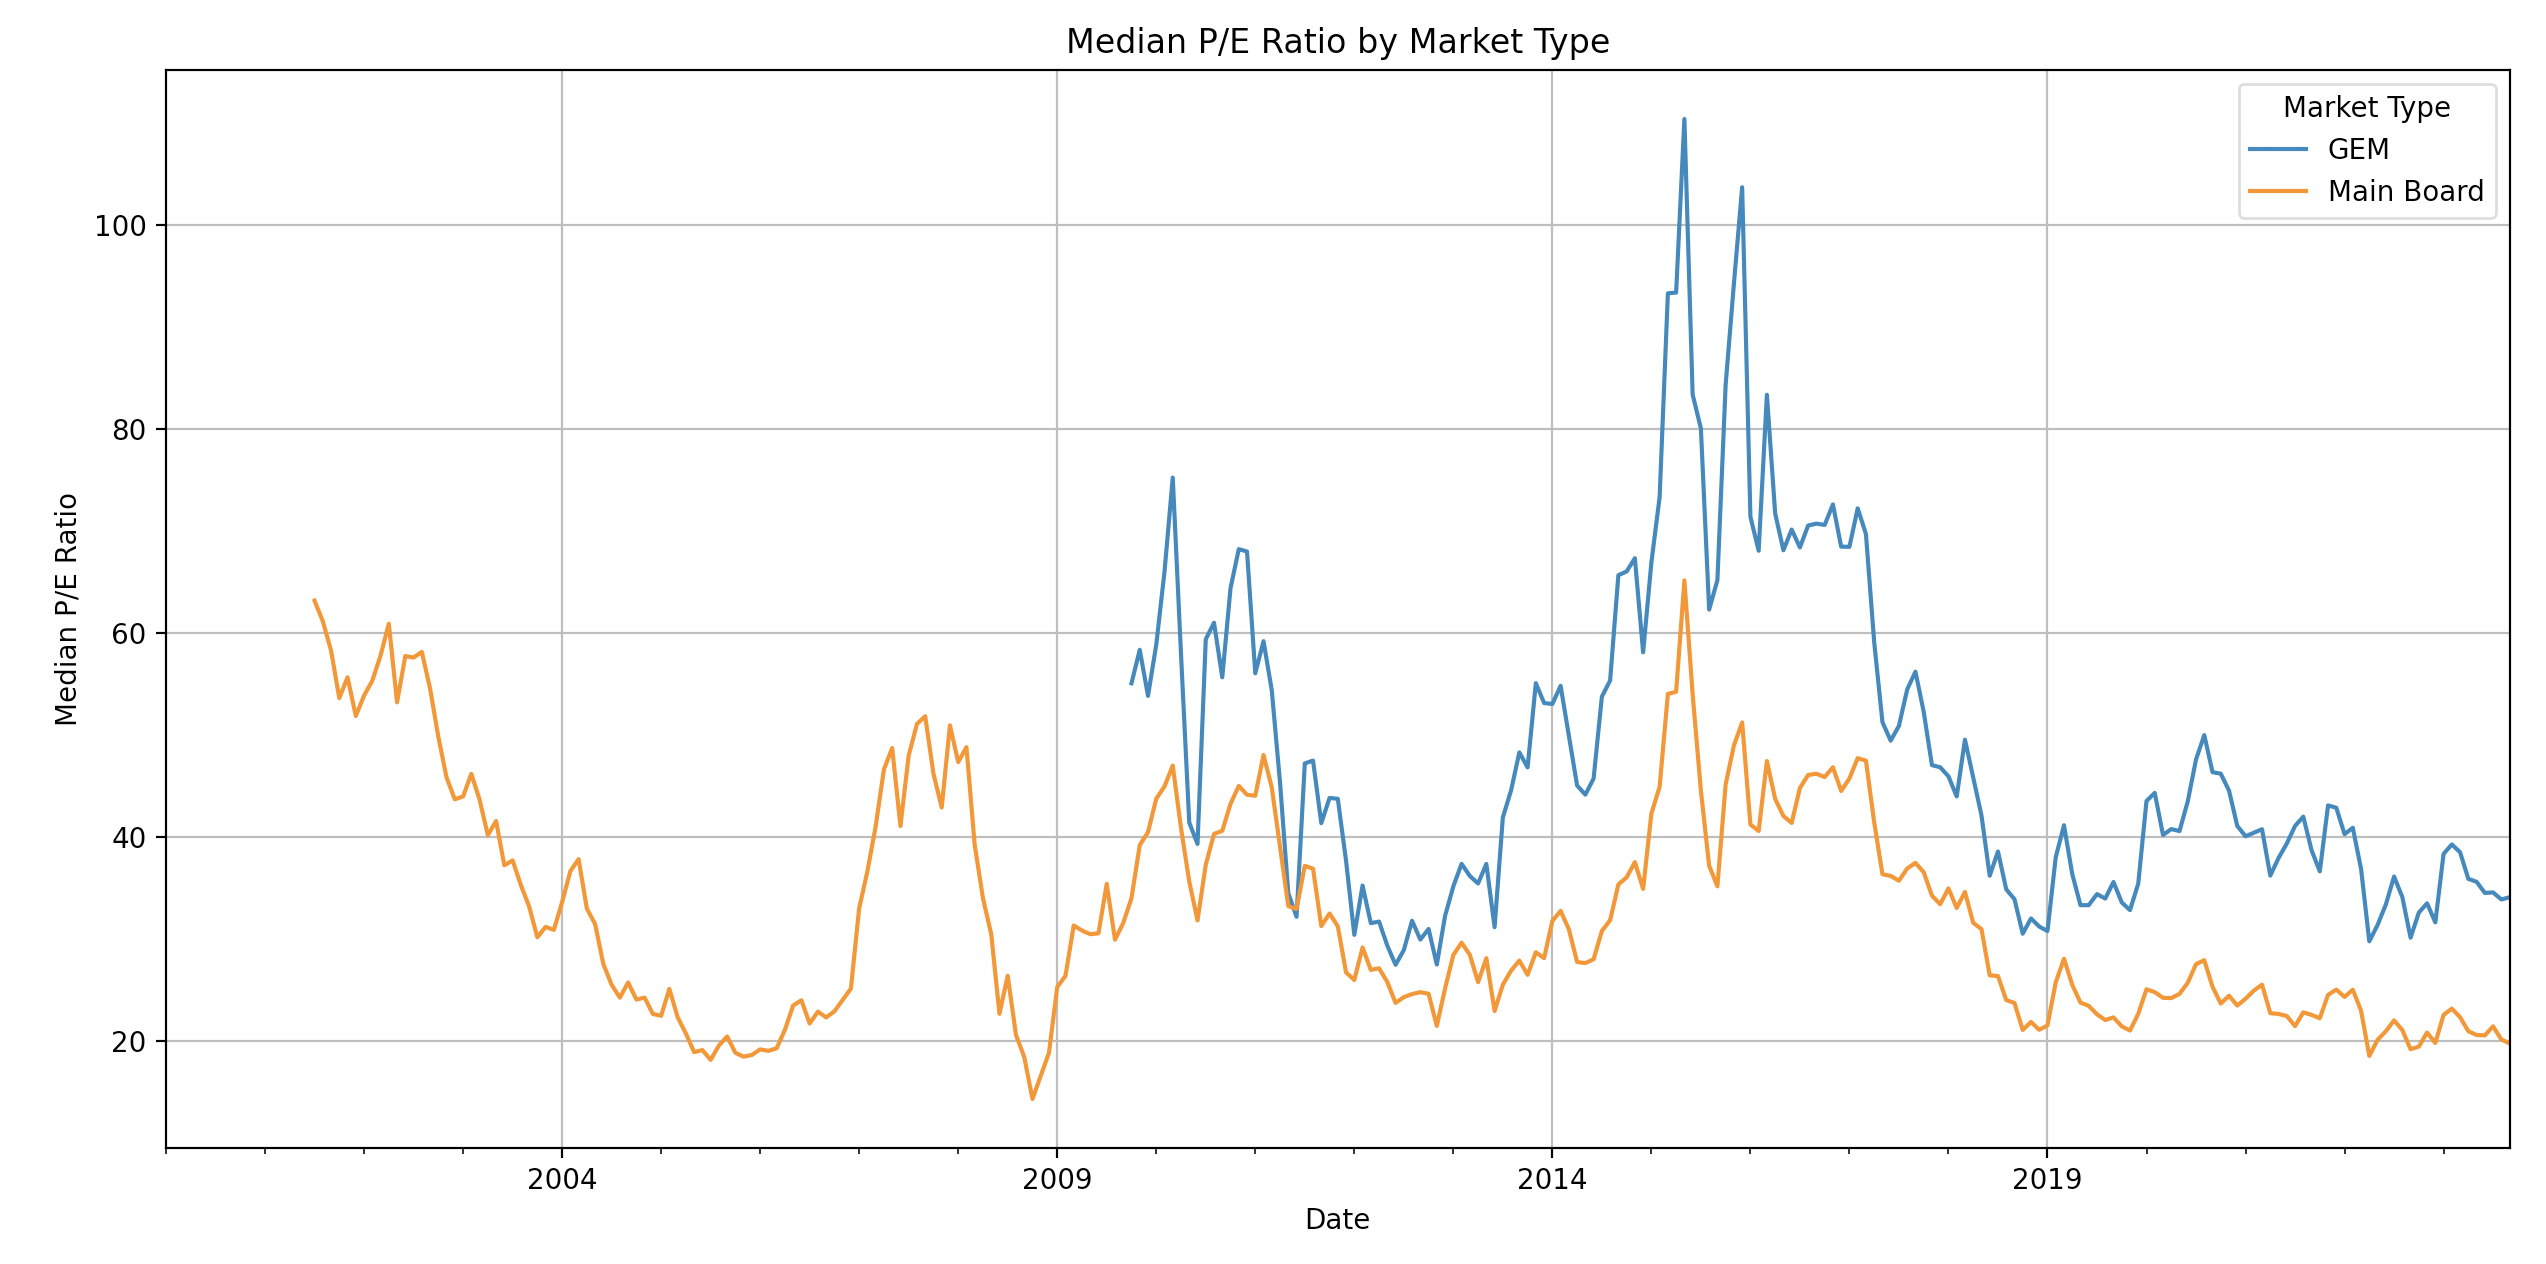
\includegraphics[width=1\textwidth]{data/median P-E TTM.png}
\caption{Time-series for Median P/E ratio by Market Type.}
\label{fig:example}
\end{figure}


\noindent
\textbf{Question (i)}

Yes. As of September 2023 (the end of the graph), it's recommended to explore new investment opportunities in both markets. The analysis of the trend line indicates that we might be at a low point, P/E ratio is really low (nearly the lowest in the history), suggesting that many companies could be undervalued at present. Historical data shows regular patterns of fluctuation, hinting at a probable future increase in market values. Therefore, entering either market now is considered a profitable move.

\noindent
\textbf{Question (ii)}

A strategy of buying or going long on index ETFs during periods of low P/E ratios and selling or shorting them during high P/E periods may be a profitable index EFF. The reason comes from the distinct patterns observed in the Price-to-Earnings (P/E) ratios, characterized by lower values on the main board and more significant fluctuations on the GEM board. Investors might also benefit from adjusting their investment allocations between the main board and GEM board based on their risk tolerance. Those open to speculation might lean towards the GEM, whereas more cautious investors might prefer the stability of the main board. 

\begin{figure}[h]
\centering
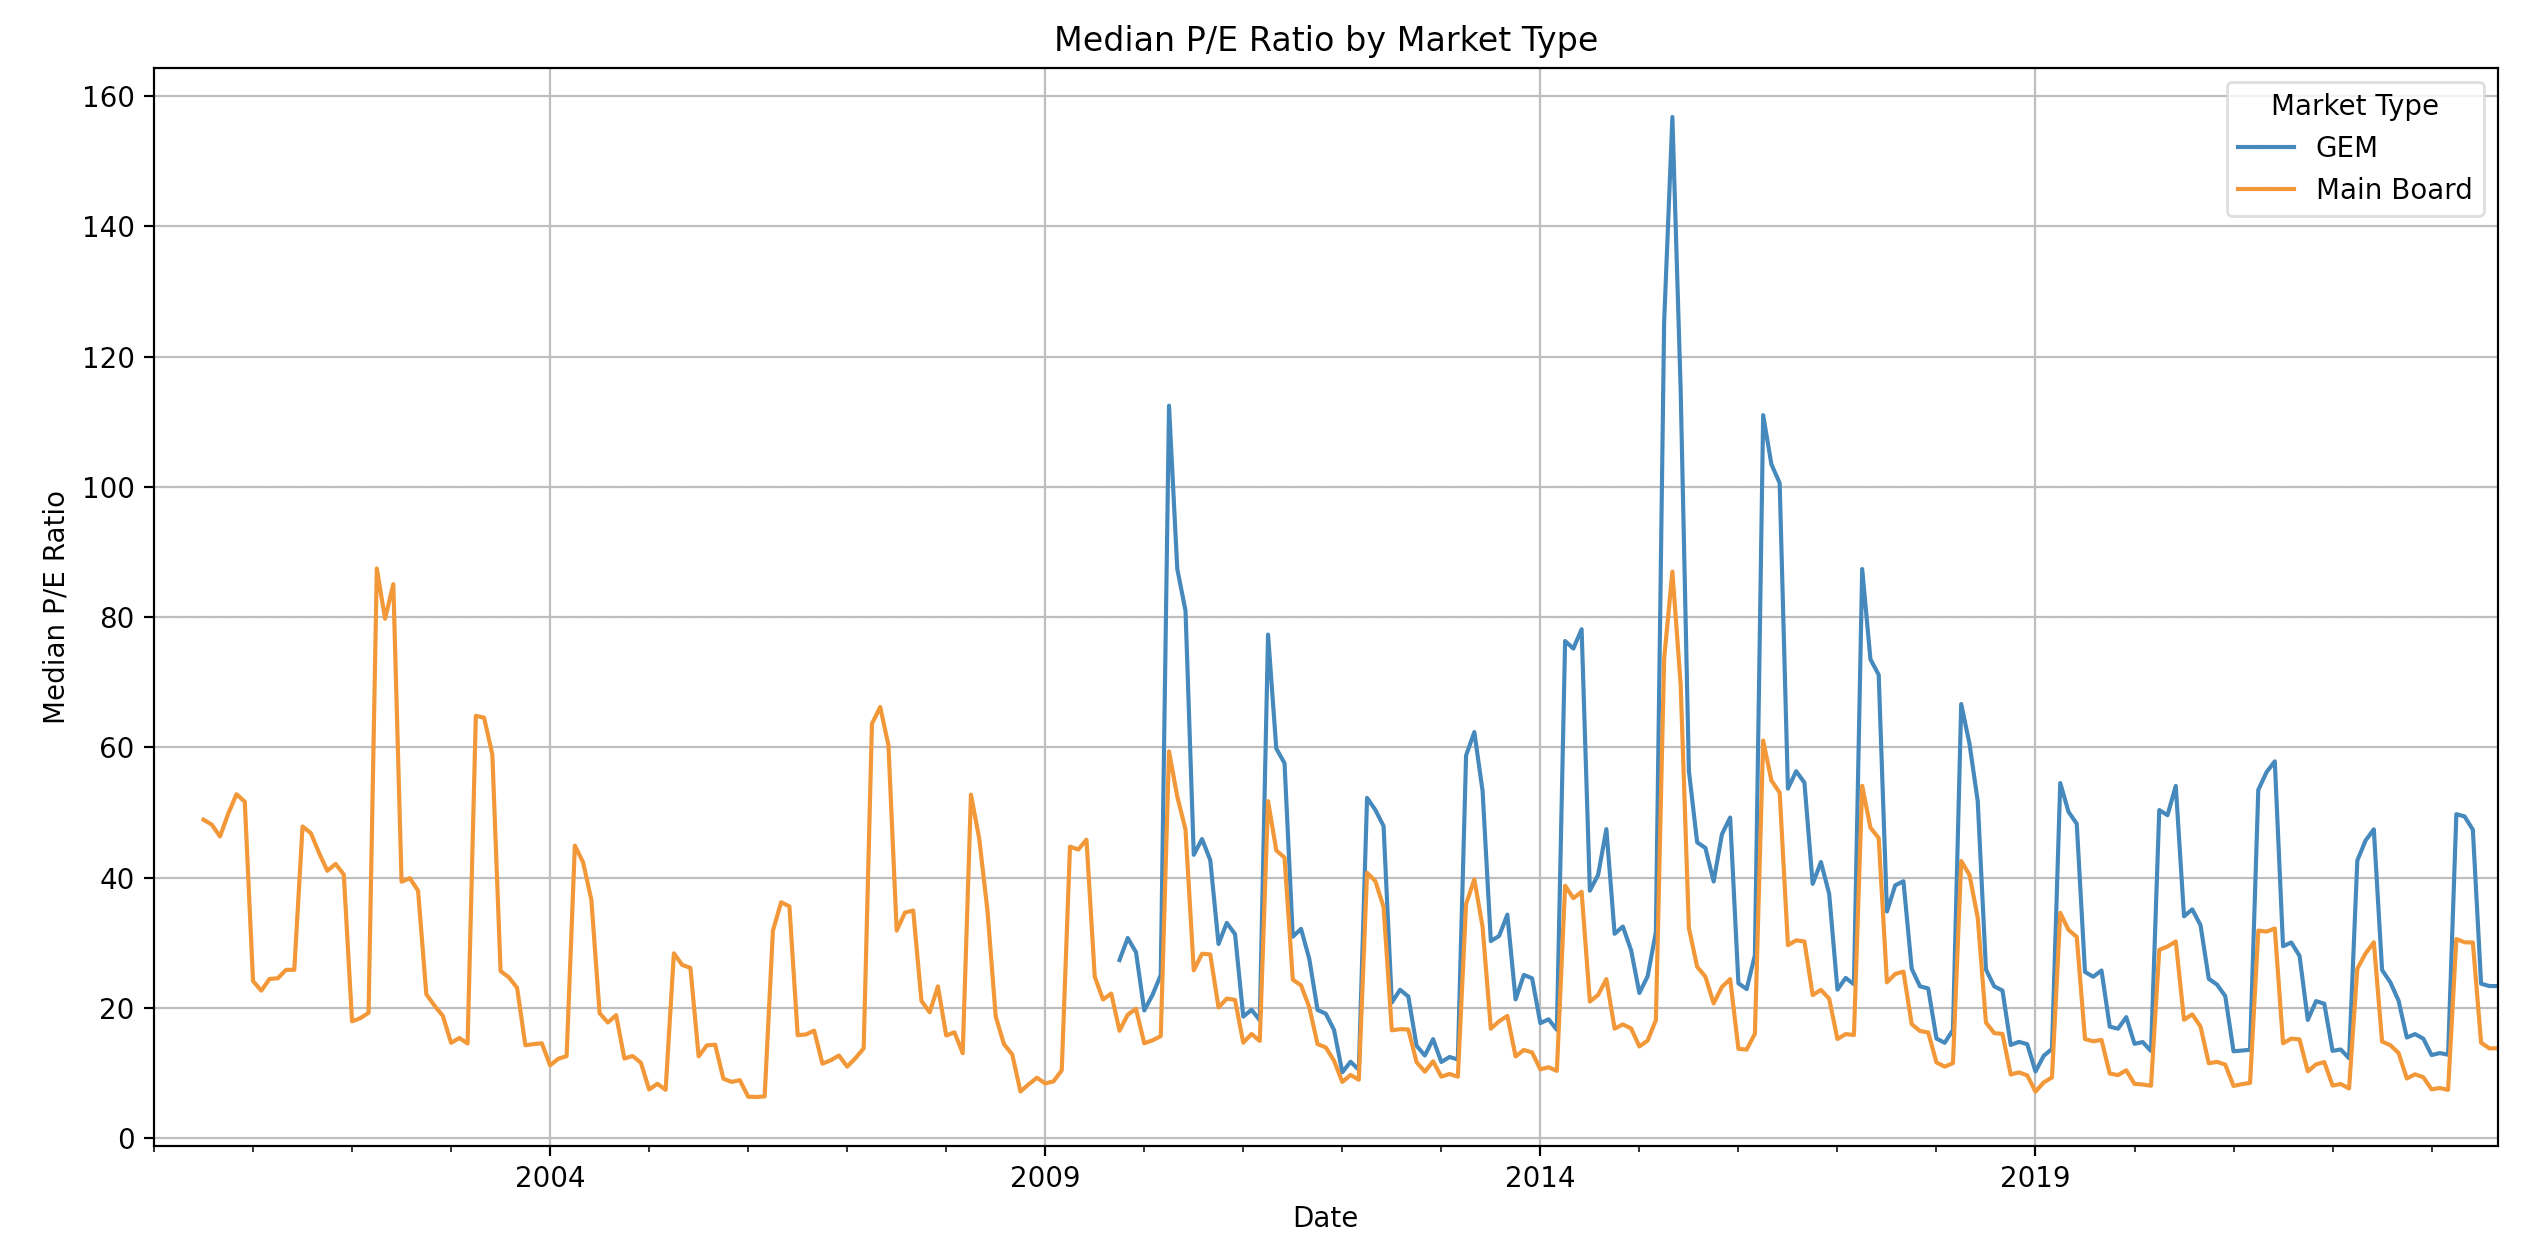
\includegraphics[width=01\textwidth]{data/median P-E 1.png}
\caption{Another Time-series for Median P/E ratio by Market Type, on non TTM EPS data.}
\label{fig:example}
\end{figure}


Based on the images obtained from non TTM EPS, the P/E ratio fluctuations in the A-share market are more pronounced, which once again strongly supports the above conclusion.